\chapter{The CMS detector and the Large Hadron Collider}
\label{c:det}
This chapter discusses the Large Hadron Collider (LHC) which is located on the Franco-Swiss border near Geneva, approximately 100~m underground at the site of the Conseil Europ\'{e}en pour la Recherche Nucl\'{e}aire (CERN)\footnote{This chapter is largely adapted from Ref.~\cite{iopdetector}}. It is a 26.7 km long synchrotron particle accelerator with four interaction points where four experiments are located. This thesis focuses on results from the Compact Muon Solenoid detector described in Section~\ref{sec:CMSdet}. The other experiments include ATLAS which is a multi-purpose experiment like CMS, the LHCb detector which focuses on the study of the physics of B hadrons, and the ALICE detector which is used to study the quark-gluon plasma. Details of the function and purpose of each of the CMS sub-detectors are given in this chapter. The algorithms which are used to reconstruct particles from the information given from the sub-detectors are given in Chapter~\ref{c:recon}.

\section{LHC}

The LHC accelerates two beams of protons which circulate in opposite directions.
This is achieved using a system of superconducting dipole magnets which have an aperture for each beam direction. Quadrapoles are used to squeeze the beam.
The protons are sourced from a bottle of hydrogen where a strong electric field is used to excite the electrons from the hydrogen atoms leaving protons behind. The protons are then accelerated through the linear accelerator LINAC2, where they reach an energy of 50~MeV. The LINAC2 works by using radio frequency cavities to charge cylindrical conductors and the protons are attracted by negative conductors and repelled by positive conductors, which boost them forward. From LINAC2, the protons are accelerated by the Proton Synchrotron Booster (PSB) to 1.4~GeV, then they are accelerated by the Proton Synchrotron (PS) to 25~GeV. This is followed by a boost to 450~GeV in the Super Proton Synchrotron (SPS), which is the final accelerator before the protons are injected into the LHC ring where their final collision energy can be achieved. 
% Each accelerator stage boosts the protons to a higher energy before they can be injected into the LHC where their final collision energy can be achieved.


The protons are accelerated in bunches which are collided at the interaction points of each experiment. This results in many collisions per bunch crossing despite the fact that many protons will miss each other and continue to be accelerated around the LHC. The background of particles coming from the frequent less interesting collisions is called \emph{pileup} (PU).

\begin{figure}[ht!]
\centering
    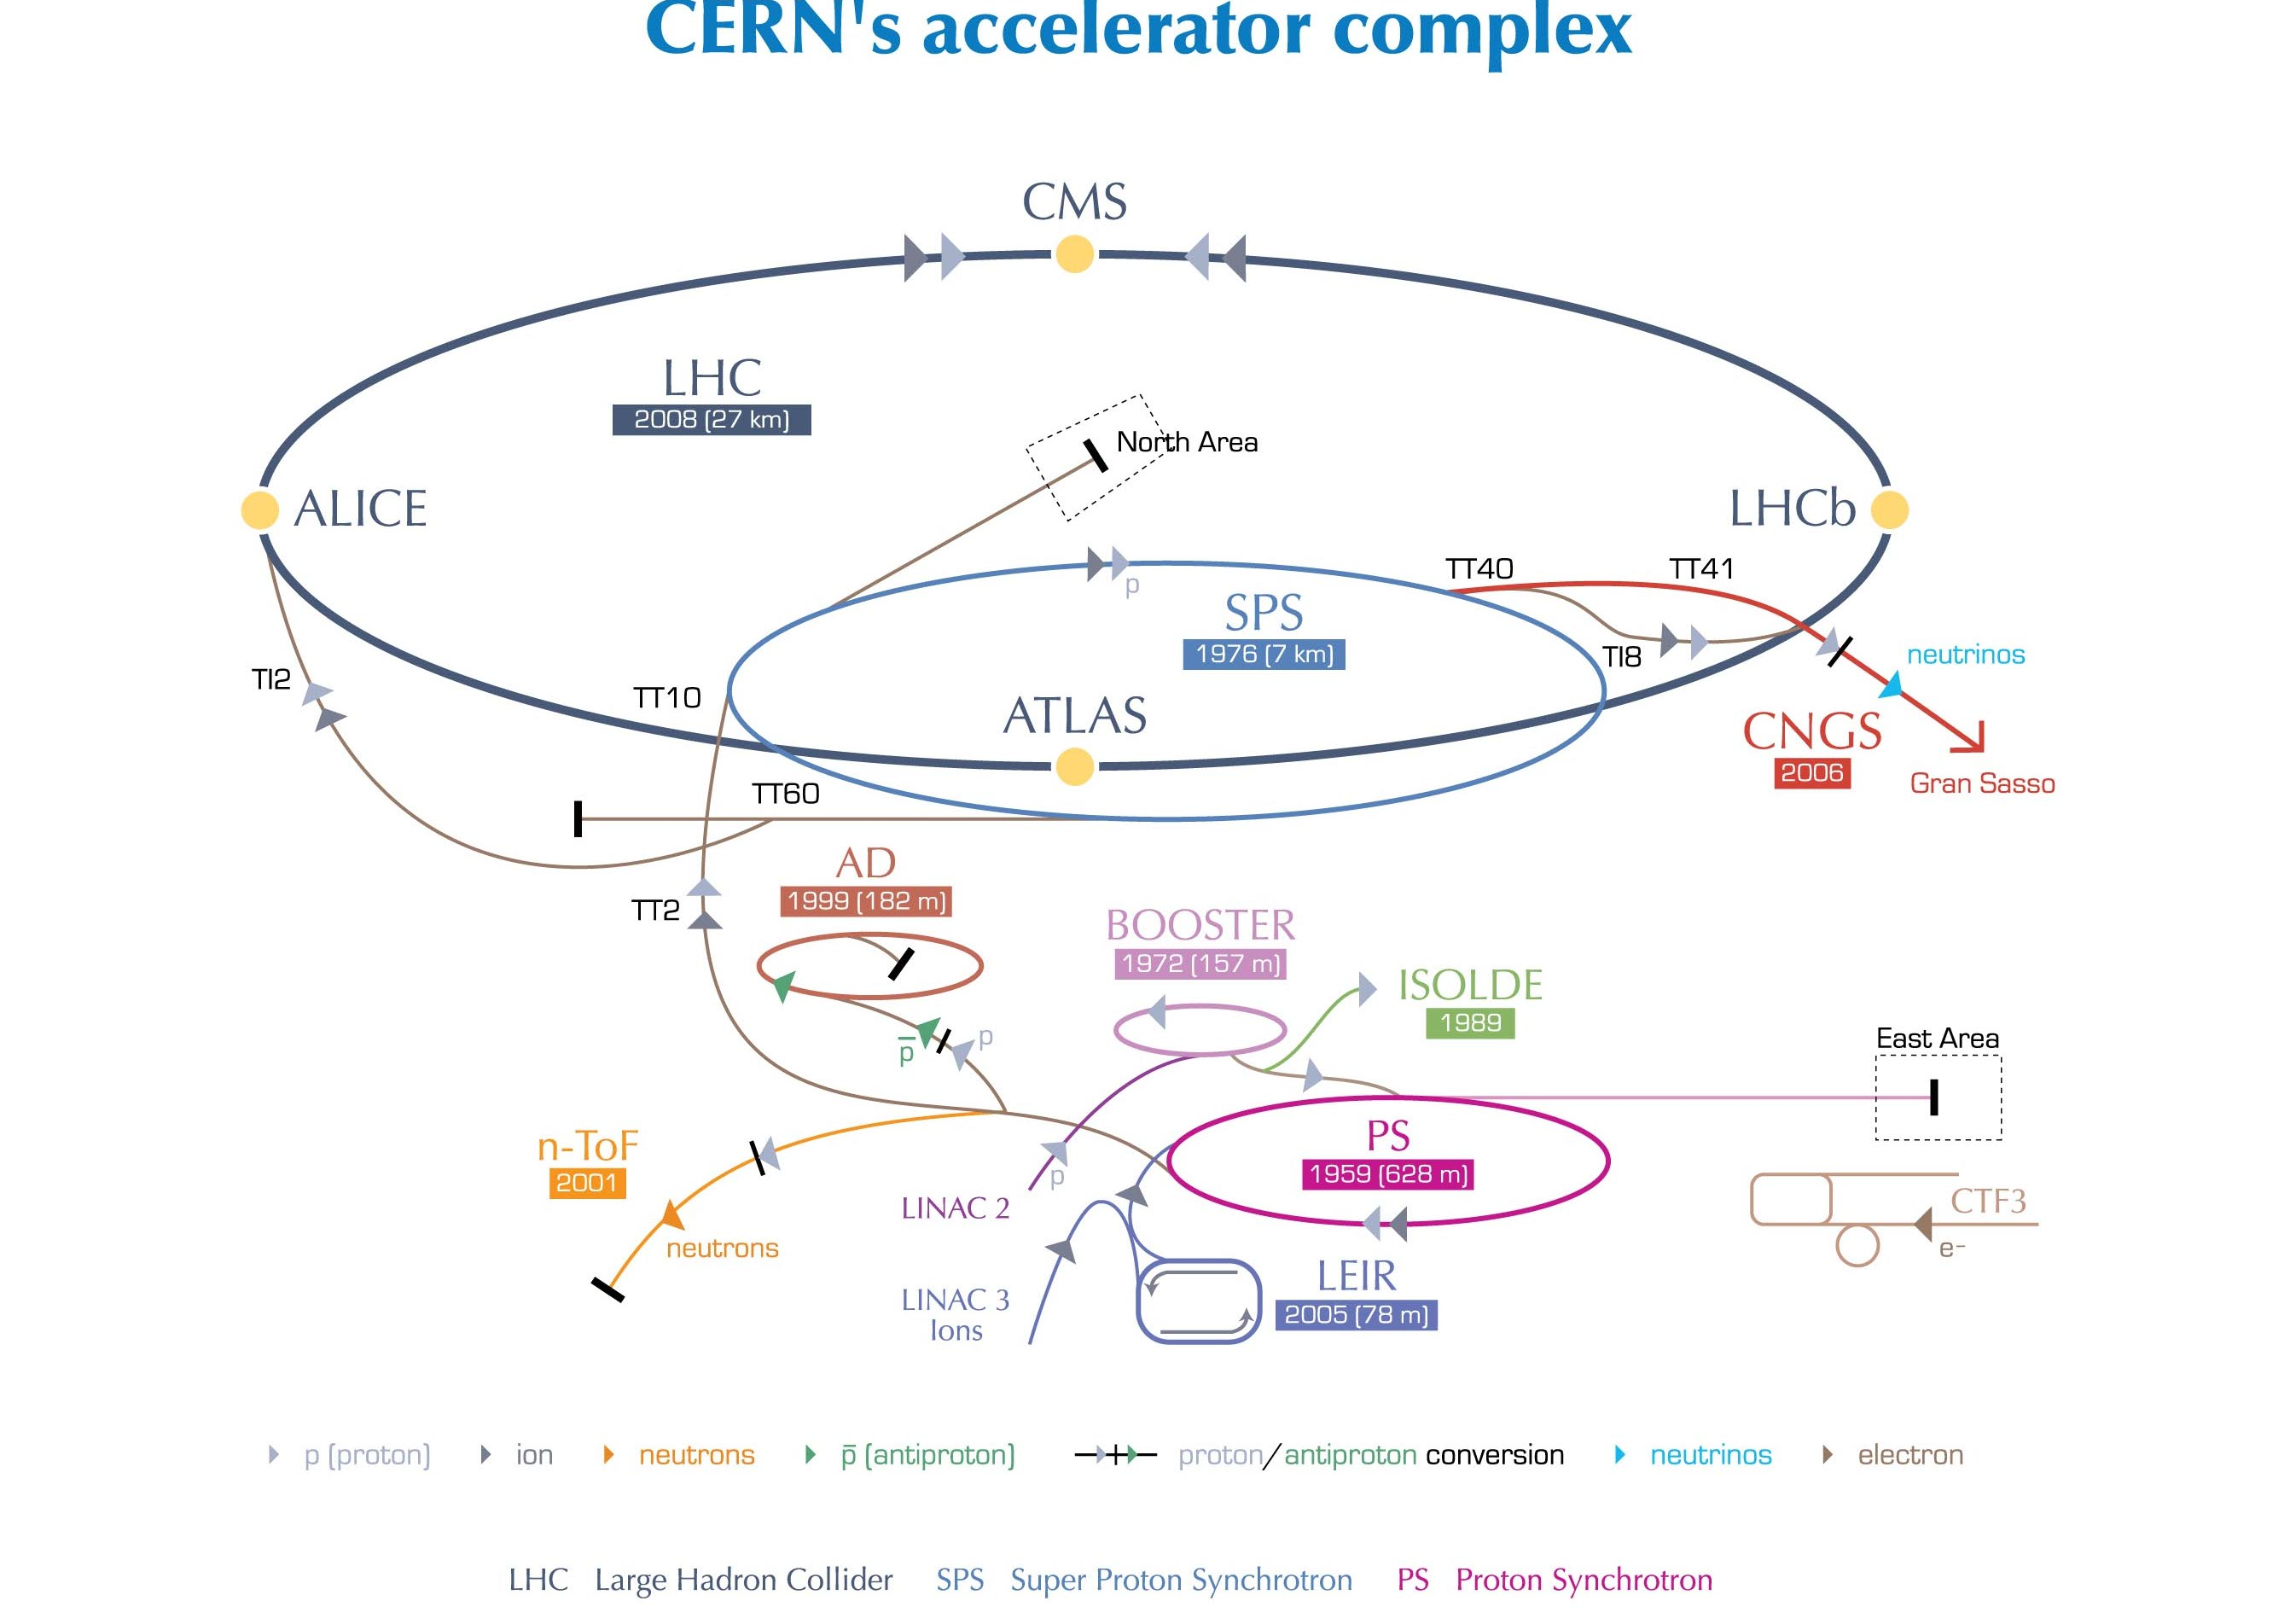
\includegraphics[width=0.95\textwidth]{images/LHCacc.jpg}
    \caption{The LHC accelerator complex at CERN. Protons are accelerated from LINAC 2 into the BOOSTER synchrotron. From there they are further accelerated in the proton synchrotron (PS) and super proton synchrotron (SPS) before finally being injected in two counter-rotating beams in the large hadron collider (LHC). The beams are crossed at the four experiments: CMS, LHCb, ATLAS and ALICE~\cite{Marcastel:1621583}.}
    \label{fig:LHC acc}
\end{figure}


The \emph{Luminosity} (\lumi) is a measure of the instantaneous collision rate and can be calculated using Eq.~\ref{eqn:lumi1}, where $f$ is the bunch frequency, and $N_1$ and $N_2$ are the numbers of particles in each bunch. The effective collision area is $4\pi\sigma_{x}\sigma_{y}$ where $\sigma_{x}$ and $\sigma_{y}$ are the $x$ and $y$ components of the beam, transverse to the beam direction. It is assumed that each beam has the same cross section.

\begin{equation}
\lumi = \frac{f{N}_{1}{N}_{2}}{4\pi\sigma_{x}\sigma_{y}}
\label{eqn:lumi1}
\end{equation}

The \emph{integrated luminosity} (\lumiint) which is shown in Fig~\ref{fig:Lumi} for the CMS experiment from 2010 until 2016 for proton-proton collisions is the delivered luminosity integrated over time. The number of events, $N_{\textrm{events}}$, produced for a particular particle physics process can be calculated from the cross section, $\sigma$, using Eq.~\ref{eqn:lumi2}.

\begin{equation}
N_{\textrm{events}} = \lumiint \times \sigma
\label{eqn:lumi2}
\end{equation}

\begin{figure}[ht!]
\centering
    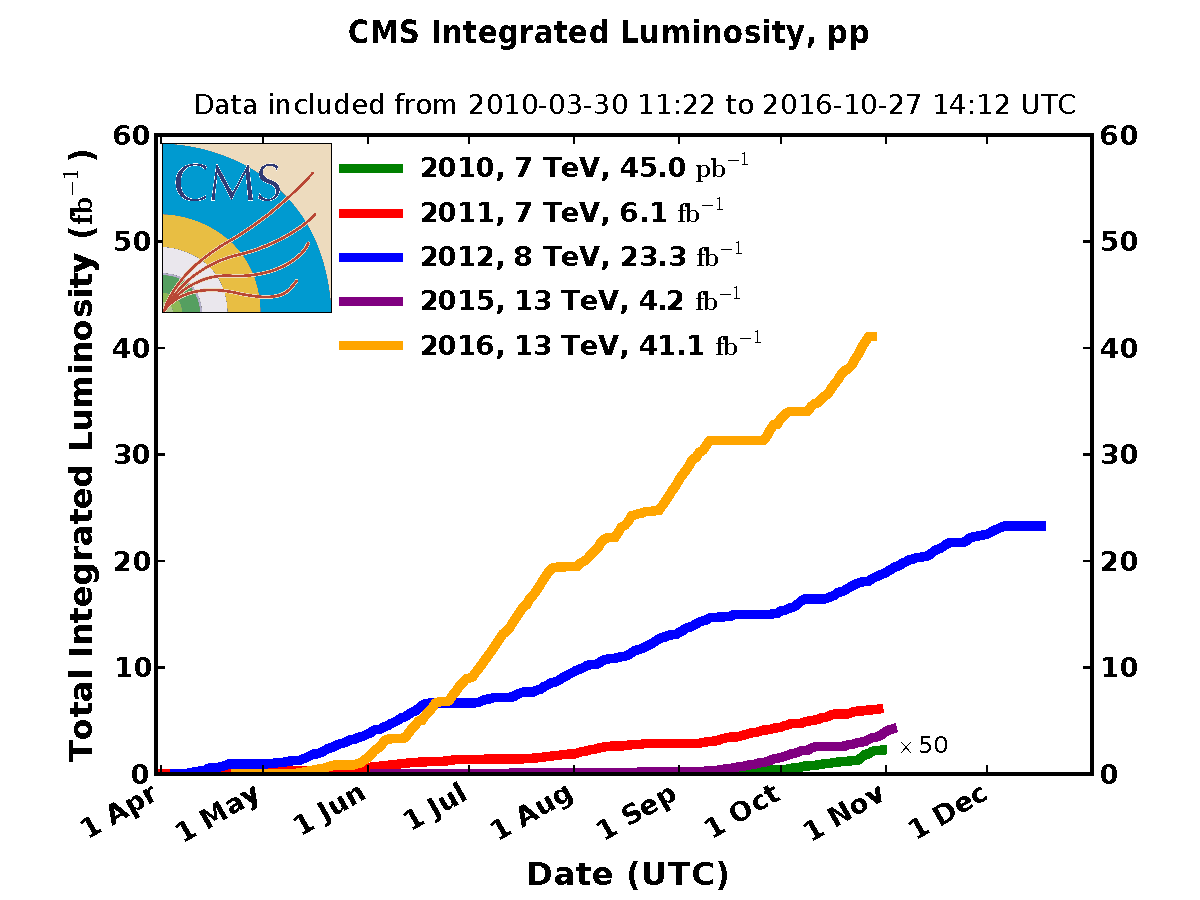
\includegraphics[width=0.95\textwidth]{images/int_lumi_cumulative_pp_2.pdf}
    \caption{The integrated luminosity in \fbinv for proton-proton collision at the CMS experiment from 2010 to 2016~\cite{lumiplotref}.}
    \label{fig:Lumi}
\end{figure}

The LHC was designed to have a centre of mass collision energy of $\sqrt{s} = 14~\TeV$. The intention was to start the machine with a lower energy in September 2008 and to obtain $\sqrt{s} = 10~\TeV$ by the end of 2008. However, an electrical fault 10 days into operation in October 2008 caused damage to over 50 of the superconducting magnets. The LHC was shut down for repairs until November 2009 when LHC achieved the record breaking 1.18 TeV per beam. The centre of mass energy was then ramped up to $\sqrt{s} = 7~\TeV$ in 2011. In 2012 this was increased to $\sqrt{s} = 8~\TeV$ and a dataset with an integrated luminosity of $\approx 20~\fbinv$ was recorded. This dataset from the run phase known as `\runone' was used for the analysis in Chapter~\ref{c:Run1}. In 2013 after \runone, Long~Shutdown~1 (LS1) commenced to make upgrades to the LHC and the detectors to allow the machine to run at $\sqrt{s} = 13~\TeV$ for `\runtwo'. \runtwo began in March 2015 and results from \runtwo are the focus of the analysis in Chapter~\ref{c:Run2}.

\runone saw the great success of the discovery of the Higgs boson, one of the main objectives of the LHC~\cite{Aad20121,Chatrchyan201230}. In \runtwo, the search for new physics continues where precision measurements will test the predictions of the SM. The CMS and ATLAS detectors are considered to be general-purpose detectors which can be used to test many areas of physics within and beyond the standard model. This includes searches for dark matter, supersymmetric particles, vector-like-quarks, lepton-flavour-violating processes, light Higgs and charged Higgs bosons, and studies of the properties of the Higgs boson such as the couplings and rare decay modes.

% \runone saw the great success of the discovery of the Higgs boson, one of the main objectives of the LHC~\cite{Aad20121,Chatrchyan201230}. In \runtwo, the search for new physics continues where precision measurements, such as the search for the production of four top quarks, will test the predictions of the SM. The CMS and ATLAS detectors are considered to be general-purpose detectors which can be used to test many areas of physics within and beyond the standard model. This includes searches for dark matter, supersymmetric particles, vector-like-quarks, lepton-flavour-violating processes, light Higgs and charged Higgs bosons, and studies of the properties of the Higgs boson such as the couplings and rare decay modes.

\section{CMS detector \label{sec:CMSdet}}

The CMS detector is a hermetic detector with a large magnetic solenoid which causes charged particles to follow a curved trajectory as they traverse the detector. Closest to the beam line is the silicon tracker which makes the most accurate position measurements. Next are the calorimetry systems for electromagnetic and separately for hadronic particles. All of these detectors are contained within the magnetic solenoid. The muon chambers are outside the solenoid where they detect muons, which are much more penetrating than other particles. The cylindrical coordinate system of the detector is defined as follows: the $x$-axis points towards the centre of the LHC ring, the $y$-axis points upwards and the $z$-axis points along the beamline in the anti-clockwise direction. The azimuthal angle $\phi$ is measured in the $(x,y)$ plane clockwise from the $x$ axis. The polar angle $\theta$ is measured clockwise from the $z$-axis. More commonly the pseudorapidity, defined in Eq.~\ref{eqn:eta}, is used instead of $\theta$.

\begin{equation}
    \eta = - \ln \left[ \tan \left(\frac{\theta}{2} \right) \right]
    \label{eqn:eta}
\end{equation}

\begin{figure}[ht!]
\centering
    \includegraphics[width=0.95\textwidth]{images/cmsdetector3.pdf}
    \caption{The CMS detector~\cite{1742-6596-513-2-022032}.}
    \label{fig:CMSdetector}
\end{figure}


\subsection{Magnetic Solenoid}

The superconducting magnetic solenoid at the core of CMS was designed to have a magnetic field of 4~T. The free bore magnet has a diameter of 6.3~m and length of 12.5~m. It uses a 4-layer winding of NbTi superconductor which is required to generate this high magnetic field. The magnet is cooled within a cryostat using liquid helium to a temperature of 4.5~K. The magnetic field is returned via an iron yoke consisting of five barrel wheels and two endcaps which are made of three discs each. The outer dimension of the iron flats is 14~m. The tracker, electromagnetic calorimeter and hadronic calorimeter are constrained to be within the inner dimensions of the solenoid as can be seen in Fig.~\ref{fig:CMSdetector}. The solenoid provides a homogeneous magnetic field, which bends particle trajectories transverse to the beam direction, over the silicon tracker region shown in Fig.~\ref{fig:TrackerWhole}.
% described in Section~\ref{sec:tracker}

\subsection{Tracker \label{sec:tracker}}

The tracking system of CMS lies inside the superconducting solenoid and surrounds the interaction point. It is 5.8~m long with a diameter of 2.5~m.
Silicon detectors are used as they can provide the high granularity and fast response required to reliably reconstruct the trajectories of particles coming from the collision vertex before the next collision occurs.
% and from the secondary vertices which originate from decaying particles. 
Reconstructing secondary vertices is also particularly important for identifying jets originating from heavy flavour quarks such as bottom quarks. This is integral for distinguishing final states involving top quarks.

It is estimated that at a PU of 20 there are 1000 particles traversing the tracker at every bunch crossing. The silicon detectors have been designed to have the radiation hardness to last for the design time of ten years. The minimum material possible was used in order to reduce the amount of multiple scattering, photon conversion and bremsstrahlung.
Cooling the tracker helps to prevent thermal runaway from leakage current, hence it was cooled to 0$^{\circ}$C in \runone and -20$^{\circ}$C in \runtwo. 
The tracking system has a nominal momentum resolution of 0.7 (5.0)\% for a particle with a momentum of 1 (1000) GeV in the central region. The impact parameter resolution is around 10~$\mu$m for high momentum tracks~\cite{Khachatryan2010}.


 % However the high density of electronics means that the tracker requires cooling to 0$^{\circ}$C in \runone and -20$^{\circ}$C in \runtwo. %Cooling also helps prevent `thermal runaway' from leakage current. 
%good to limit interaction with material in tracker

The tracking system consists of two main sections: the pixel tracker makes up the innermost section and the strip tracker surrounds the pixel tracker as seen in Fig.~\ref{fig:TrackerWhole}. 

\begin{figure}[ht!]
\centering
    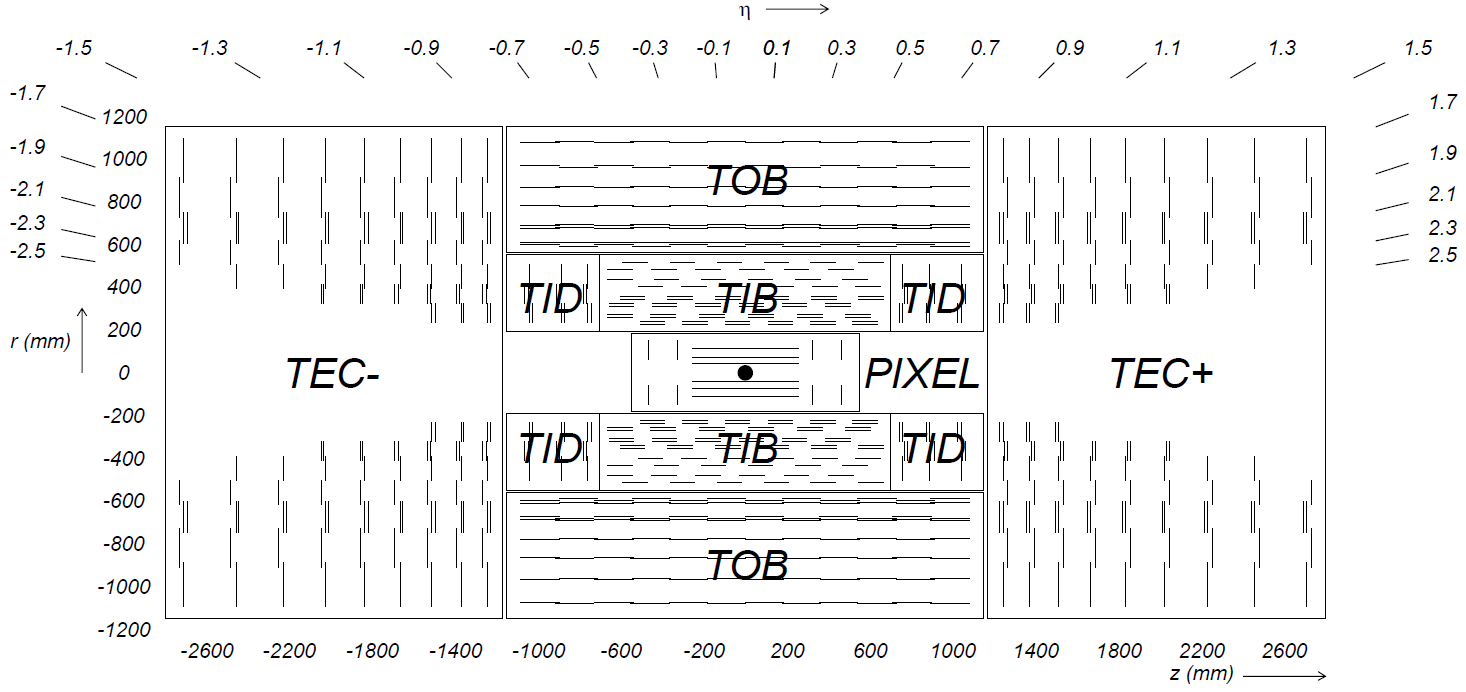
\includegraphics[width=0.95\textwidth]{images/TrackerWhole.png}
    \caption{The tracking system~\cite{1748-0221-3-08-S08004}.}
    \label{fig:TrackerWhole}
\end{figure}

\textbf{Pixel tracker}\\
As the pixel detector is closest to the interaction vertex, it experiences the highest flux of particles at $\approx$ 1~MHz per~mm$^{2}$. The fine granularity of the pixel detector (100 x 150~$\mu$m in $(r-\phi)$x$(x-z)$) is required in order to keep the occupancy below 1\%. It consists of three barrel layers which range between 4.0~cm and 10.2~cm from the interaction point and 2 disks which are transverse to the beamline as seen in Fig.~\ref{fig:TrackerWhole}.\\

\textbf{Strip tracker}\\
Two types of silicon strip tracker are used. Closest to the interaction point (20~-~50~cm) are the tracker inner barrel detectors (TIB) which contain silicon micro-strips (10~cm x 80~$\mu$m). An occupancy of $\approx$ 2-3\% is achieved for a fluence of $\approx$ 60~kHz per~mm$^{2}$.
An increased strip pitch of 180$~\mu$m can be used in the tracker outer barrel (TOB) due to the lower fluence of 3~kHz per~mm$^{2}$. To cover the larger surface area, the effective strip length is increased to 25 cm. However, increased strip length increases the noise. To combat this the strips are made thicker to 500~$\mu$m compared to 320~$\mu$m in the TIB.
The tracker inner disk (TID) and tracker end cap (TEC) have strips which are aligned radially to the beamline with a strip pitch of 80$~\mu$m and 200$~\mu$m, respectively. The TID and TEC extend the tracker acceptance to $\abs{\eta}<2.5$.

\subsection{Electromagnetic Calorimeter}

The electromagnetic calorimeter (ECAL) is a homogeneous, hermetic detector made up of 61200~(7324) lead tungstate, PbWO$_{4}$, crystals in the barrel (endcap) region. In the barrel region the light from these scintillating crystals is collected in avalanche photodiodes and in the endcap region by vacuum phototriodes. The barrel region covers $\abs{\eta}<1.479$ whilst the two semi-circular `Dees' which make up the endcaps extend the range to $\abs{\eta}<3.0$.



Good resolution can be obtained from PbW0$_{4}$ crystals and they are fast and radiation resistant. Equation~\ref{eqn:ECALres} shows the dependence of the resolution on the energy of the particle, E. The stochastic term for the statistical fluctuations on the number of secondary particles produced is represented as $S$. The noise from the electronics and digitisation is given by $N$ and the constant term $C$ arises from calibration errors and leakage of the shower outside of the calorimeter. 
\begin{equation}
\left(\frac{\sigma}{E}\right)^2 = \left(\frac{S}{\sqrt{E}}\right)^2 + \left(\frac{N}{E}\right)^2 + C
\label{eqn:ECALres}
\end{equation}
For an electron test beam with no magnetic field and no material between the beam and the ECAL, the parameters in Eq.~\ref{eqn:ECALres} were measured to be $S=0.028$,$N=0.12$~GeV and $C=0.0003$~\cite{1748-0221-2-04-P04004}. This gives an energy resolution of $\approx~0.5\%$ for a 100~GeV particle.

The crystals have a high density and small radiation length ($X_{0}=0.89$~cm) so that the ECAL can be compact. Another importantly quality is that they are optically clear allowing all fo the light to be collected. The scintillation decay time is comparable to the time between bunch crossings with 80\% of light being emitted within 25~ns. The crystals have a tapered shape in the barrel region and lie parallel in the endcap region. The crystals are 1.29~m from the beam line in the barrel region and 3.15~m from the the interaction point in the longitudinal direction in the endcap region. The crystals are contained in thin-walled aluminium structures which make up submodules.

In the endcap region there is a preshower detector, shown in Fig.~\ref{fig:ecal}, which is a two-layer sampling calorimeter. There are two layers of lead used as a radiator material to initiate the electromagnetic shower and silicon strip detectors after each layer (orthogonal in each plane) to measure the energy depositied. The preshower detector helps to identify neutral pions and to distinguish electrons from minimum ionising particles.

\begin{figure}[ht!]
\centering
    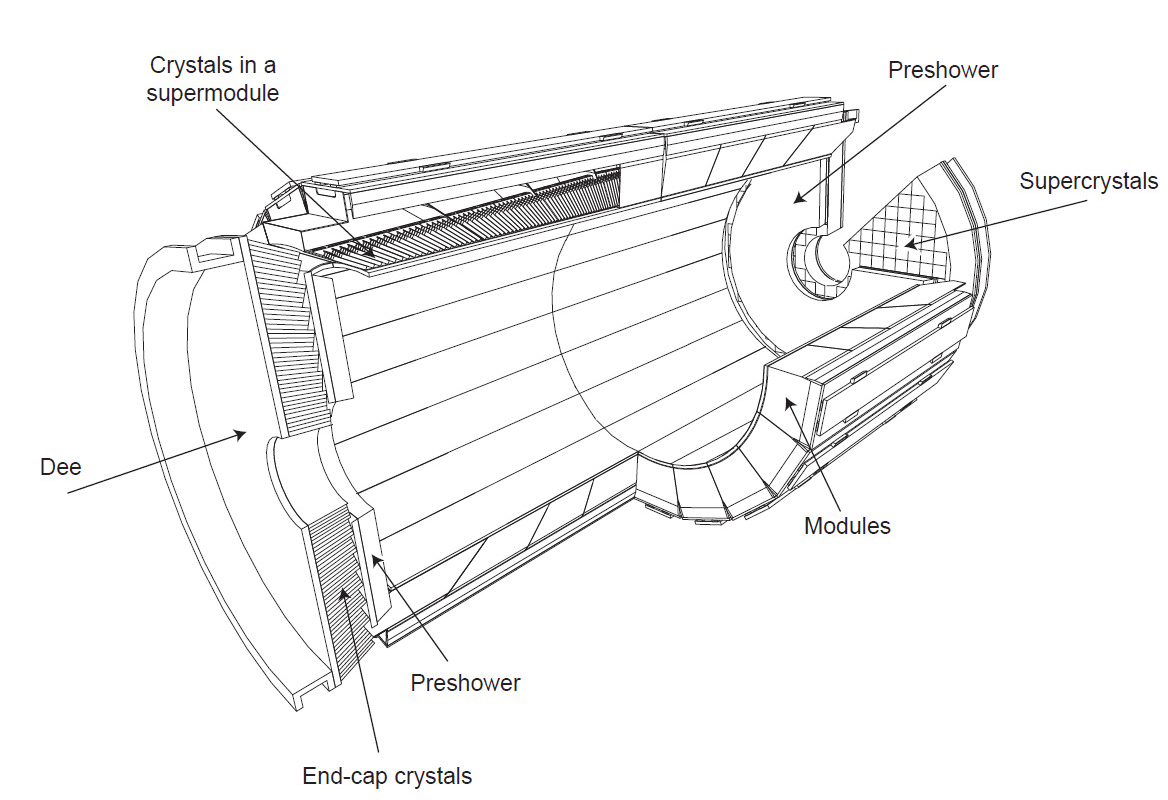
\includegraphics[width=0.95\textwidth]{images/ecal.png}
    \caption{The ECAL system where modules contain submodules and the 36 supermodules are made up of four modules each. The supercrystals are made up of groups of 5 x 5 crystals in the endcap~\cite{Isildak:2013kfa}.}
    \label{fig:ecal}
\end{figure}

\subsection{Hadron Calorimeter}

The hadron calorimeter (HCAL) is used for identifying hadron jets. It has barrel (HB) and endcap (HE) regions made up of sampling calorimeters which have coverage of $\abs{\eta}<1.3$ and $1.3<\abs{\eta}<3.0$, respectively. The HB and HE are placed between the ECAL and solenoid magnet, and therefore are restricted to the radial dimensions, R, of 1.77~m $<$ R $<$ 2.95~m. The barrel consists of two halves, HB+ and HB-, which are composed of 36 wedges made up of 14 flat brass absorber plates parallel to the beam axis, alternated with plastic scintillator. Stainless steel plates are used for the innermost and outermost plates to provide structural support. The HE has a similar system of alternating absorber and plastic scintillator.
Due to their restricted dimensions the HCAL and ECAL do not always contain all of the energy from the particle showers. Therefore another detector known as the outer hadronic calorimeter (HO) is embedded in the muon system which lies outside of the solenoid magnet to measure the energy leakage from the HCAL and ECAL.
The forward HCAL extends the range from $\abs{\eta}<2.3$ to $\abs{\eta}<5.2$ such that very forward jets can be detected. The hermeticity of the detector ensures a good coverage on detecting the total hadronic energy and hence good resolution can be obtained on missing transverse energy which could come from neutrinos or BSM particles.

\begin{figure}[ht!]
\centering
    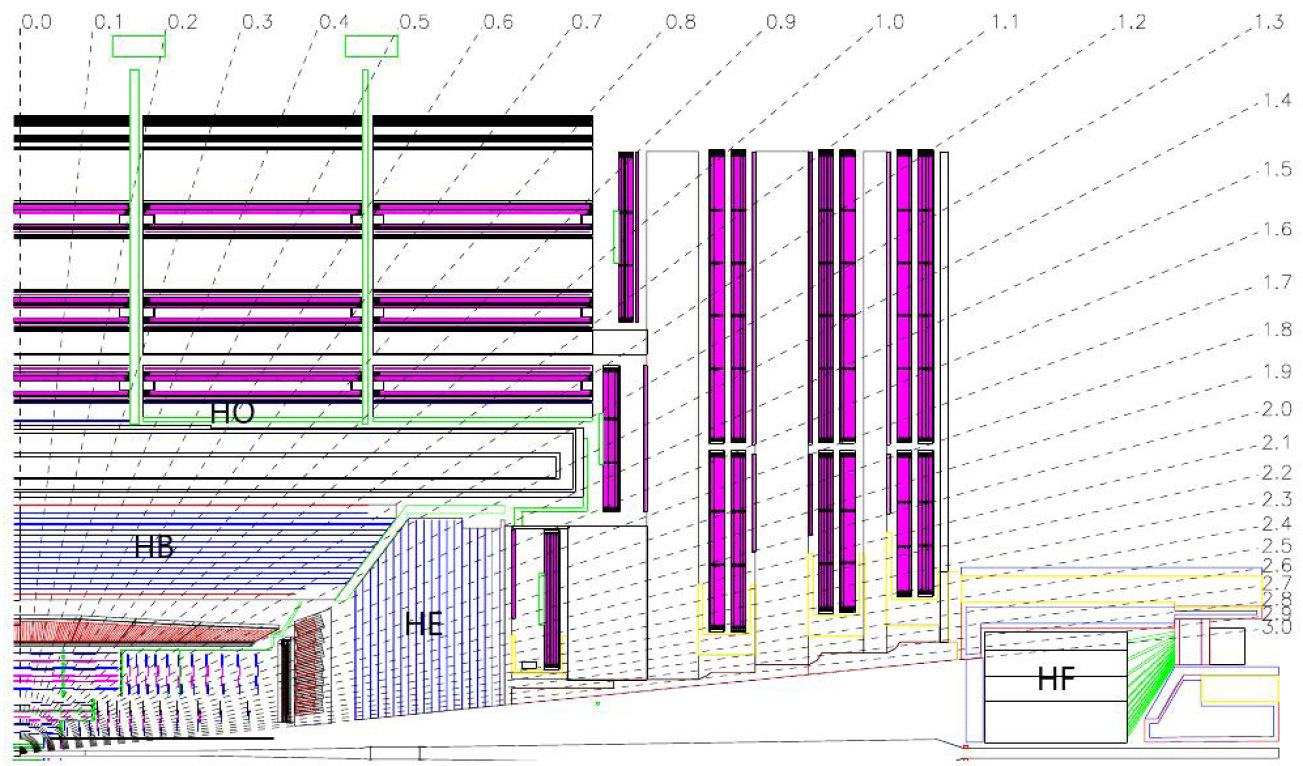
\includegraphics[width=0.95\textwidth]{images/HCAL.png}
    \caption{The HCAL system~\cite{Isildak:2013kfa}.}
    \label{fig:hcal}
\end{figure}

The energy resolution of the HCAL for neutral hadronic particles is $120\%/\sqrt{E (GeV)}$~\cite{Beaudette:2014cea}. Neutral hadronic interactions are the most important consideration for the energy resolution of the HCAL as, unlike charged particles, no additional information can be obtained from the tracker to combine with the calorimetry measurement to reduce the resolution.

\subsection{Muon Chambers}
As the name CMS suggests, muon identification and measurement was a central focus in the design of the detector. The muon chambers are interspersed within the iron flux return yoke. These thick layers of iron act as a hadron absorber. Muons are much less affected by radiative losses through the detector material than electrons, therefore they are able to penetrate through to the outermost layers of the detector. Figure~\ref{fig:muonchamber} shows the layout of the muon chambers around the detector. 
\begin{figure}[ht!]
\centering
    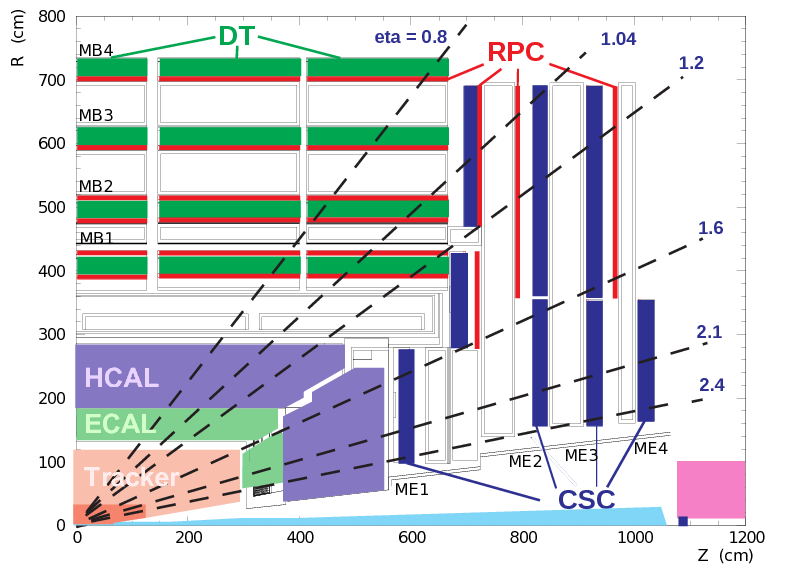
\includegraphics[width=0.95\textwidth]{images/MuonChambers.png}
    \caption{The muon chamber system~\cite{Kim:2012ix}.}
    \label{fig:muonchamber}
\end{figure}
The muon chambers consist of a cylindrical barrel section and 2 planar endcaps. The magnetic field is uniform in the barrel region where drift tubes (DT) are arranged into chambers, some of which make measurements in $r-\phi$ and some of which make measurements in $z$. This provides a high efficiency for matching individual hits in different stations to one single muon track.
In the endcaps, where the muon flux is high and the magnetic field is non-uniform, cathode strip chambers (CSC) are used due to their fine segmentation, fast response and radiation resistance. The CSC stations are aligned perpendicular to the beam line and are positioned between the flux return plates. The cathode strips are positioned as radial lines and the anode wires run perpendicular to the cathode strips. Together they can measure the position in $r-\phi$ and $\eta$. The CSCs provide robust pattern recognition for matching hits to other stations and to the tracker as well as for rejecting non-muon backgrounds. 
Together the barrel and end-cap region provide uninterrupted coverage up to $|\eta|<2.4$.\\
Resistive plate chambers (RPC) are added in the barrel and endcap sections of the muon chambers. They consist of two parallel plate chambers which sandwich readout strips, known together as a double-gap module. The sum of the two signals from each gap creates one total induced signal. There are six RPCs in the barrel section and there are three layers of RPCs in the endcap.
Where ambiguous tracks exist due to multiple hits in the muon chambers, the RPCs can help to distinguish the correct track. They have a fast response and can time-tag an ionising event in much less than the 25 ns bunch spacing time and hence they can assign candidate tracks to the relevant bunch crossing. The resolution of the RPCs is courser than the DTs and CSCs. This courser information from the RPCs is used in the trigger which is described in the following section.

The muon chamber measurements provide the dominant contribution to the energy resolution for high-momentum muons. For muons with low momentum the tracker provides the dominant contribution to the energy resolution when the tracks are more curved. At around 1~TeV both systems provide a momentum resolution of $\approx5\%$. Figure~\ref{fig:muonres} shows the muon transverse momentum resolution gained from using only the muon system, only the tracking system, and the combination of the two. It can be seen that above 200~GeV the combination of the information from the muon system with the tracking system improves the overall resolution compared to using the tracking system only.
\begin{figure}[ht!]
\centering
    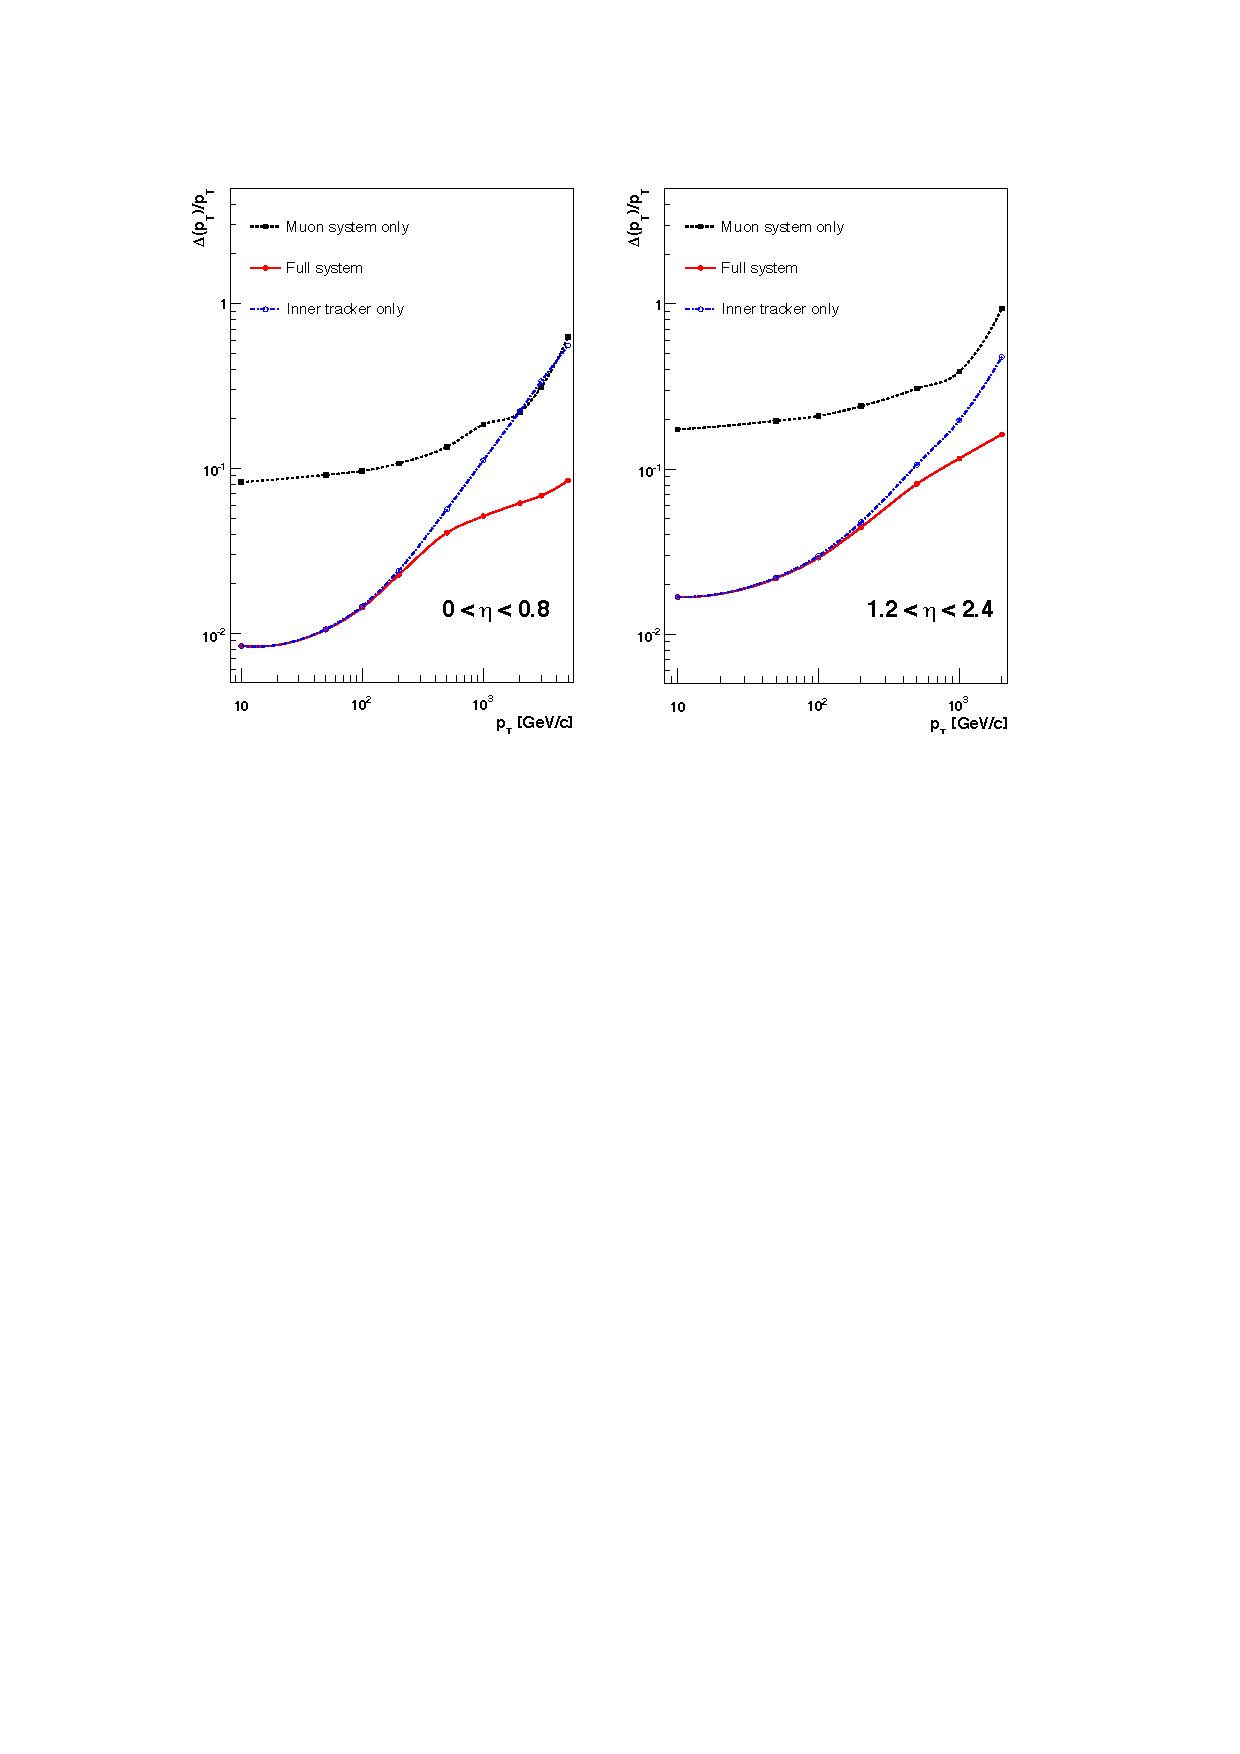
\includegraphics[width=0.95\textwidth]{images/muon_resolution.pdf}
    \caption{The muon transverse momentum resolution as a function of transverse momentum (\pt) using the muon system only (black), the inner tracking only
  (blue), and both (red), in regions of \abs\eta \num{<0.8} (left) and \num{1.2} $<$\abs\eta\num{<2.4} (right)~\cite{1748-0221-3-08-S08004}.}
    \label{fig:muonres}
\end{figure}


\subsection{Trigger \label{det:trigger}}
As each of the subdetectors have now been described, the remaining hardware and software which collects the information for analysis can now be discussed. The amount of information which can be stored is much less than the amount produced within the subdetectors. Collisions occur at a rate of 40 MHz (beam crossing interval of 25 ns). The rate reduction capability of the trigger system was designed to reduce the rate by at least a factor of $10^5$. This occurs in two main stages, the Level-1 (L1) trigger and High-Level Trigger (HLT). The L1 trigger is composed of highly programmable custom electronics, mainly FPGAs. ASIC and programmable memory lookup tables are used where higher speed and radiation hardness is required closer to the beam spot. Full high resolution data is held in the front-end electronics whilst the L1 trigger decides whether or not to keep the event based on courser information from the calorimeters and muon chambers. The HLT is a software based filter farm ($\approx$ 1000 processors) which has access to all of the readout data from the subdetectors. The HLT can assesses more complex information in order to filter out less interesting events and categorise the most interesting ones. 

\subsection{Upgrades for \runtwo}

In LS1, repairs were made to the LHC magnet splices to allow safe operation at the design energy of $\sqrt{s} = 14~\TeV$. All of the detectors on the LHC ring were able to make essential repairs and upgrades. For CMS this included repairing damaged silicon pixels and strips in the tracker and inserting the tracker back into CMS with better centering around the beam line. The temperature of the tracker was lowered to -20$^{\circ}$C to mitigate against radiation damage. In the ECAL the EE and ES subsystems underwent minor repairs. New photodetectors were added to the HO in the HCAL to improve the signal to noise ratio. The main change to the muon systems has been to the RPCS with the addition of the fourth disk (RE4). For the muon system CSCs, 72 chambers have been added to the existing 468 chambers. In addition to the detector upgrades, improvements have been made to the trigger and DAQ.

These upgrades have allowed CMS to operate at $\sqrt{s} = 13~\TeV$ in 2015 with the smaller bunch spacing of 25~ns compared to the previous 50~ns bunch spacing in \runone.

\subsection{Data collections}

The data quality monitoring (DQM) group monitor incoming data online by reconstructing a small subset of the data immediately to ascertain whether all sub-detectors in CMS are operational. Offline they go through several stages of DQM as the data are reprocessed and reconstructed. Data which has been collected while all sub-detectors were working, the magnet is at full field and the beam conditions are stable is certified by the DQM group for use in physics analyses. Hence the amount of data used for analyses is less than the total collected, as in Fig.~\ref{fig:Lumi}. Different run ranges are usually separated by short shutdowns for maintenance or they may have different run conditions such as different instantaneous luminosity~\cite{1742-6596-219-7-072020}.\\
The proton-proton collision datasets recorded by CMS and used in this thesis are given in Table~\ref{tab:run1Data} for the \runone data that is used in Chapter~\ref{c:Run1} and in Table~\ref{tab:run2Data} for the \runtwo data that is used in Chapter~\ref{c:Run2}. 
\begin{table}[ht!]
\centering

\begin{tabular}{|l|l|l|}
\hline
Dataset                    & Recorded & $\mathcal{L}$ \pbinv \\ \hline
Single Muon Run A     & 2012     & 888                  \\ 
Single Muon Run B     & 2012     & 4436                 \\ 
Single Muon Run C     & 2012     & 7125                 \\ 
Single Muon Run D     & 2012     & 7426                 \\ \hline
Total                      &          & 19695                \\ \hline\hline
Single Electron Run A & 2012     & 876                  \\ 
Single Electron Run B & 2012     & 4420                 \\ 
Single Electron Run C & 2012     & 7132                 \\ 
Single Electron Run D & 2012     & 7294                 \\ \hline
Total                      &          & 19721                \\ \hline
\end{tabular}
\caption{\runone datasets at 8~TeV, when they were recorded and how much data was recorded.}
\label{tab:run1Data}
\end{table}


\begin{table}[ht!]
\centering

\begin{tabular}{|l|l|l|}
\hline
Dataset                    & Recorded & $\mathcal{L}$ \pbinv \\ \hline
Single Muon Run C     & 2015     & 17.2                 \\ 
Single Muon Run D     & 2015     & 2611.5               \\ \hline
Total                      &          & 2628.7               \\ \hline \hline
Single Electron Run C & 2015     & 17.2                 \\ 
Single Electron Run D & 2015     & 2611.5               \\ \hline
Total                      &          & 2628.7               \\ \hline
\end{tabular}
\caption{\runtwo datasets at 13~TeV, when they were recorded and how much data was recorded.}
\label{tab:run2Data}
\end{table}

% Upgrade in energy and 50ns to 25ns bunch\\
% L1-Trigger system-higher granularity -additional processingcapabilities, 
% upgrade photo-detectors and electronics for the hadron calorimeters\\
% (HCAL) to reduce background signals - improve measurement of jets and missing-energy
% at high PU.
% Reference to pixel detector paper with upgrades~\cite{Dominguez:1481838}

% \begin{figure}[ht!]
% \centering
%     \includegraphics[width=0.55\textwidth]{images/TrackerUpgradeXSec.png}
%      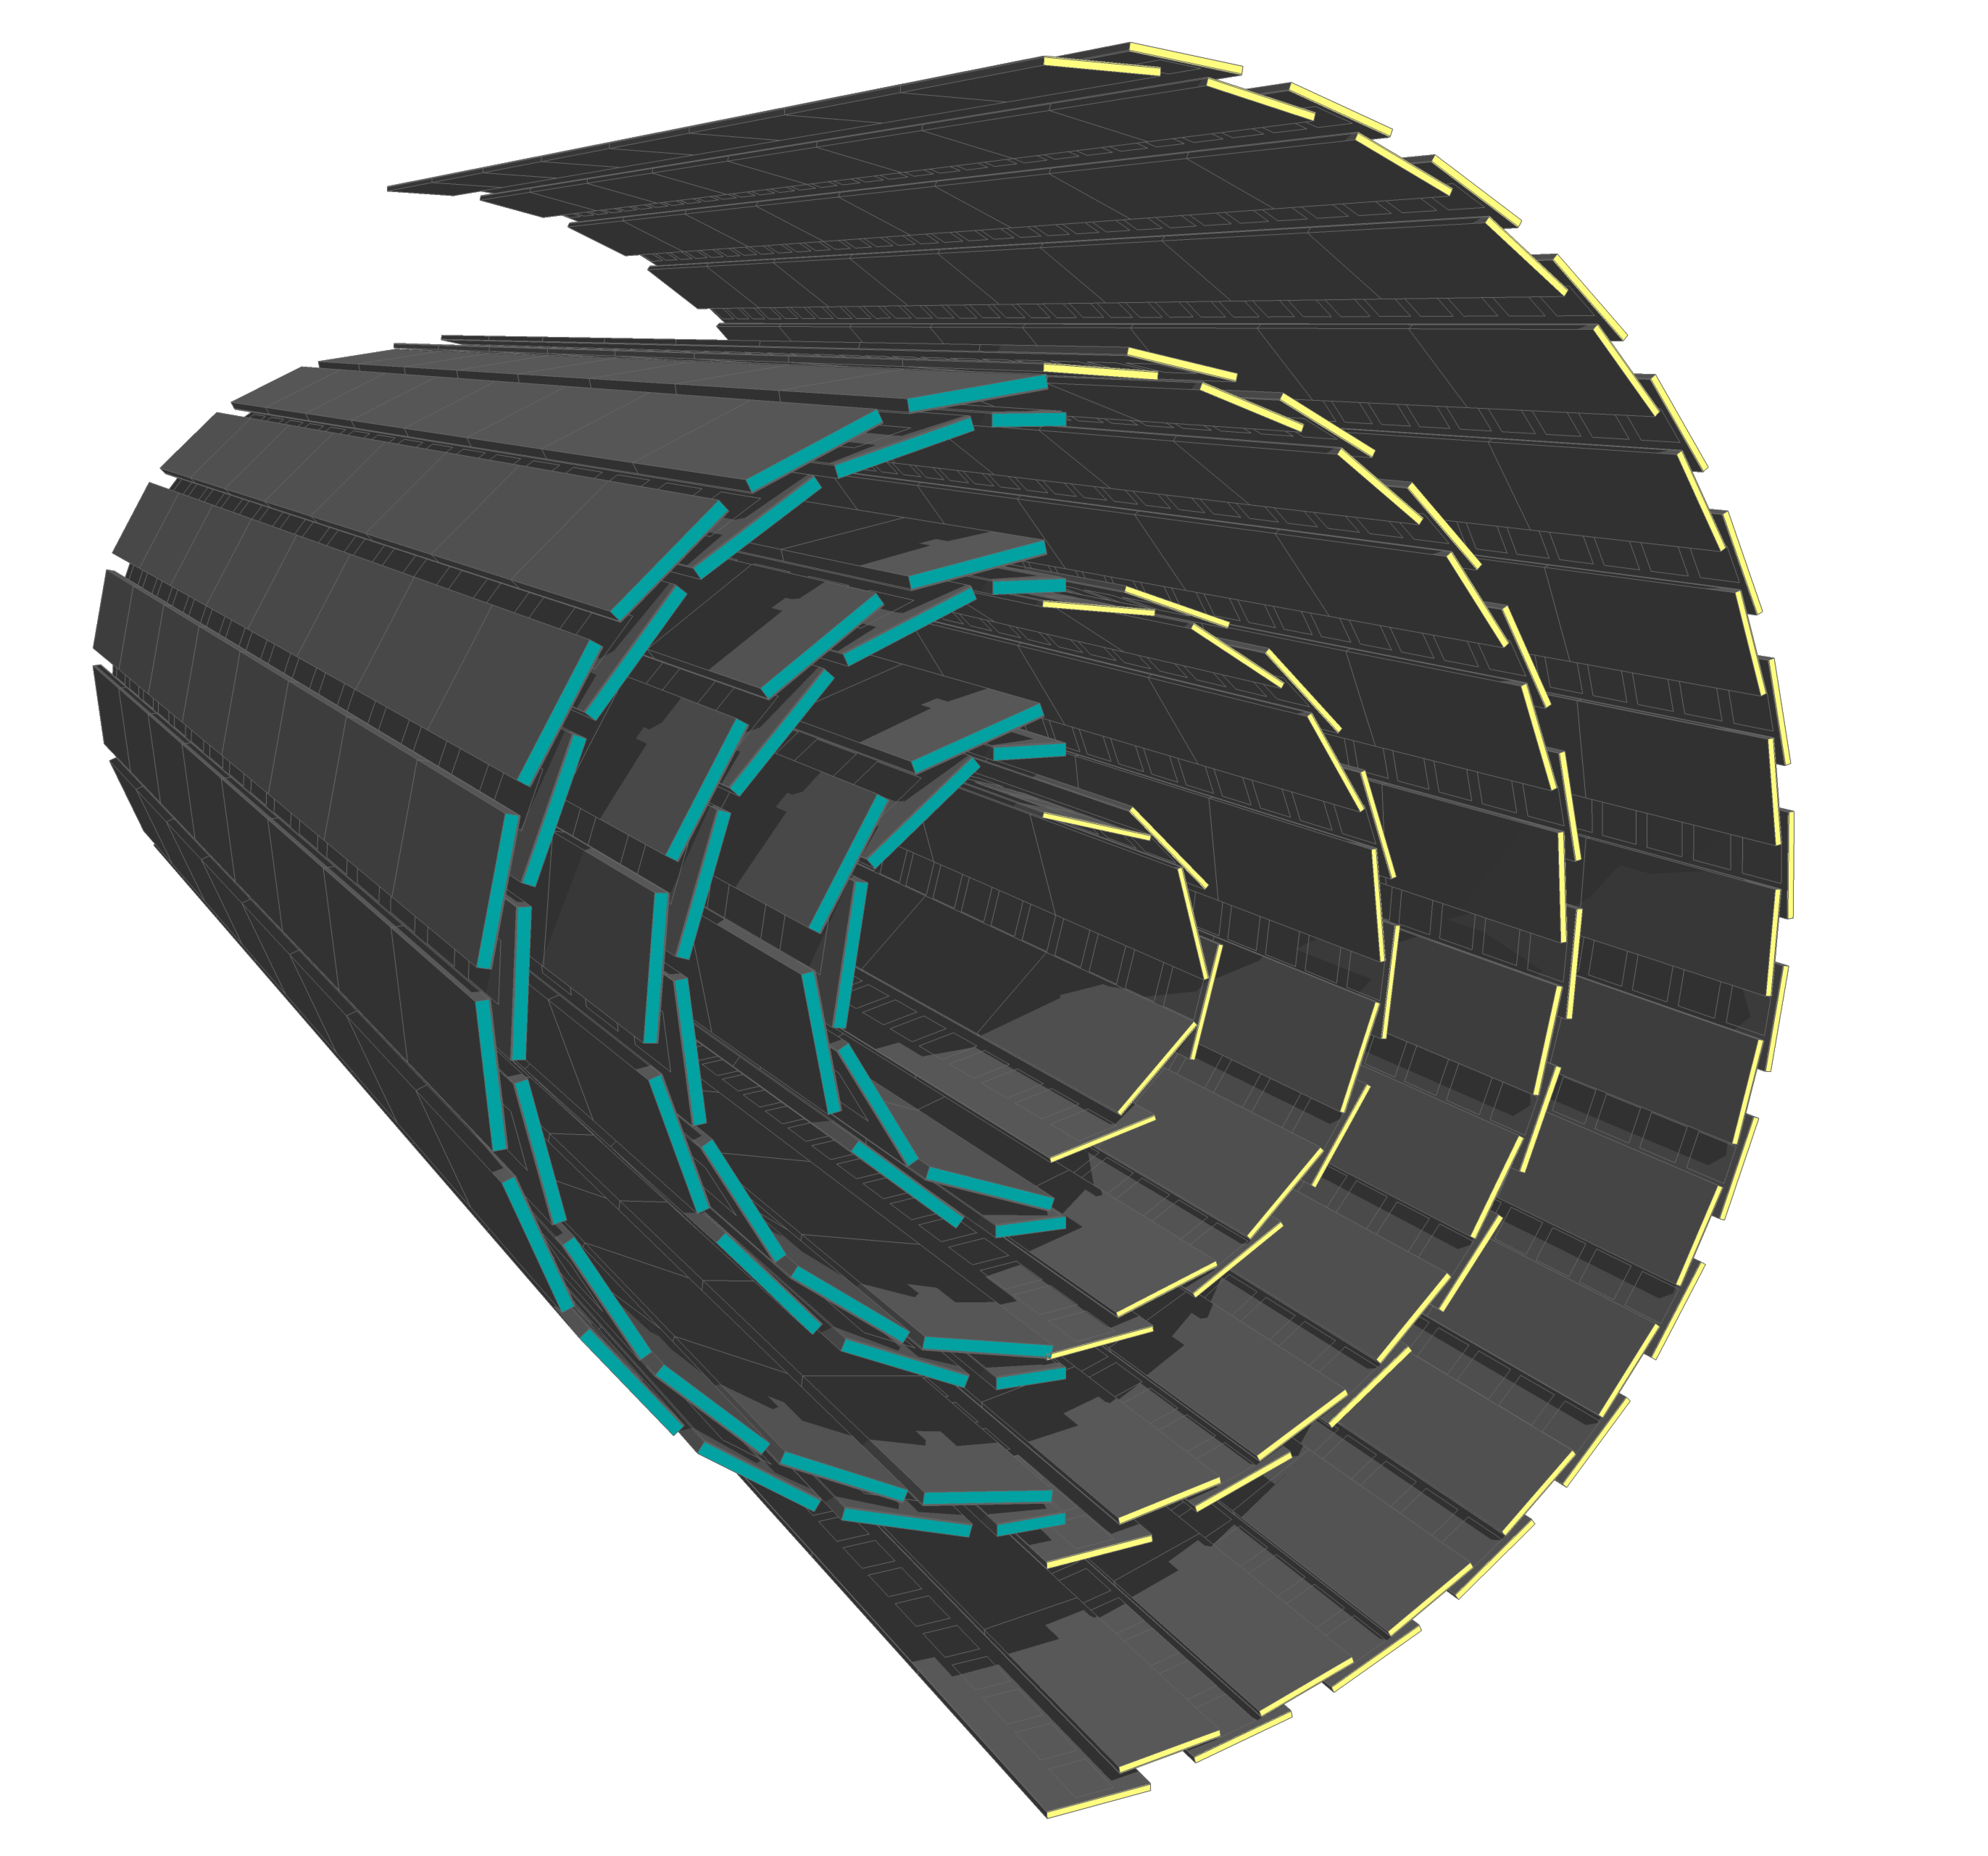
\includegraphics[width=0.42\textwidth]{images/TrackerUpgradeBarrel.png}          
%     \caption{Pixel tracker with half initial and half upgrade geometries~\cite{1742-6596-513-2-022032}}
%     \label{fig:pixel}
% \end{figure}


